\documentclass[12pt,letterpaper]{article}
%\documentstyle[11pt]{article}
\usepackage[utf8]{inputenc}
\usepackage{amsmath}
\usepackage{xfrac}
\usepackage{amsfonts}
\usepackage{amssymb}
\usepackage[version = 3]{mhchem}
\usepackage{chemstyle}
%%For Table perhaps%%
%\usepackage{graphics}
\usepackage{graphicx}
\usepackage{epstopdf}
%\usepackage{tabularx,ragged2e,booktabs,caption}
%\newcolumntype{C}[1]{>{\Centering}m{#1}}
%\renewcommand\tabularxcolumn[1]{C{#1}}
\usepackage[left=2cm,right=2cm,top=2cm,bottom=2cm]{geometry}
%\usepackage{subcaption} 
%\usepackage{caption}
\usepackage{siunitx}
\usepackage{subfig}



\begin{document}
\setlength{\parindent}{0cm} 


\frenchspacing


% Default margins are too wide all the way around. I reset them here
\setlength{\topmargin}{-.5in}
\setlength{\textheight}{9in}
\setlength{\oddsidemargin}{.125in}
\setlength{\textwidth}{6.25in}




\title {Nonlinear Curve Fitting---Lab 3 and Lab 6} 
\author {CENG 340--Introduction to Environmental Engineering\\
Instructor: Deborah Sills}
\date {September 17, 2013}
\maketitle


\section*{Overview}




\section *{Due Date}
\textbf{ Submit your memo via email before lab on September 24.} 

\section *{Learning Objectives}
\begin{enumerate}
\item Learn to fit laboratory data to mathematical models using non-linear curve fitting.\
\item Create a high-quality figure that presents data and model fits clearly.\
\item Discuss and analyze data and fitted models presented in a figure.\ 
\end{enumerate}

\section *{Rationale}
\begin{enumerate}
\item Environmental engineers use mathematical models that describe phenomena---such as aeration of an activated sludge reactor---to design treatment technologies.  Thus far you have used linear models (easy to do in Excel), but many phenomena are not linear, and linearizing non-linear data results in less accurate models.  Many computer programs (e.g., Matlab, R, KaleidaGraph, SigmaPlot) include non-linear curve fitting packages and today we will use KaleidaGraph.  
\item To be successful, engineers need to communicate results of preliminary experiments and final designs clearly and concisely to their colleagues, supervisors, and clients.  Such communications often include figures that contain graphs.  In addition to creating clear and effective figures, engineers need to discuss and analyze their figures appropriately. 
\end{enumerate}
 
\section *{In Class Preparatory Exercise: Figures--the good and the not so good}
The following two figures are taken from a document created by Prof. Malusis, called \emph{DOs and DON’Ts for Creating High-Quality Figures that Contain Graphs}.   (You will receive a copy of this document after we complete this exercise).  Both figures show the same data and model fits, but the graphs were created with different software packages and were formatted differently.\\

\pagebreak
%\begin{figure}[h]
%\centering
%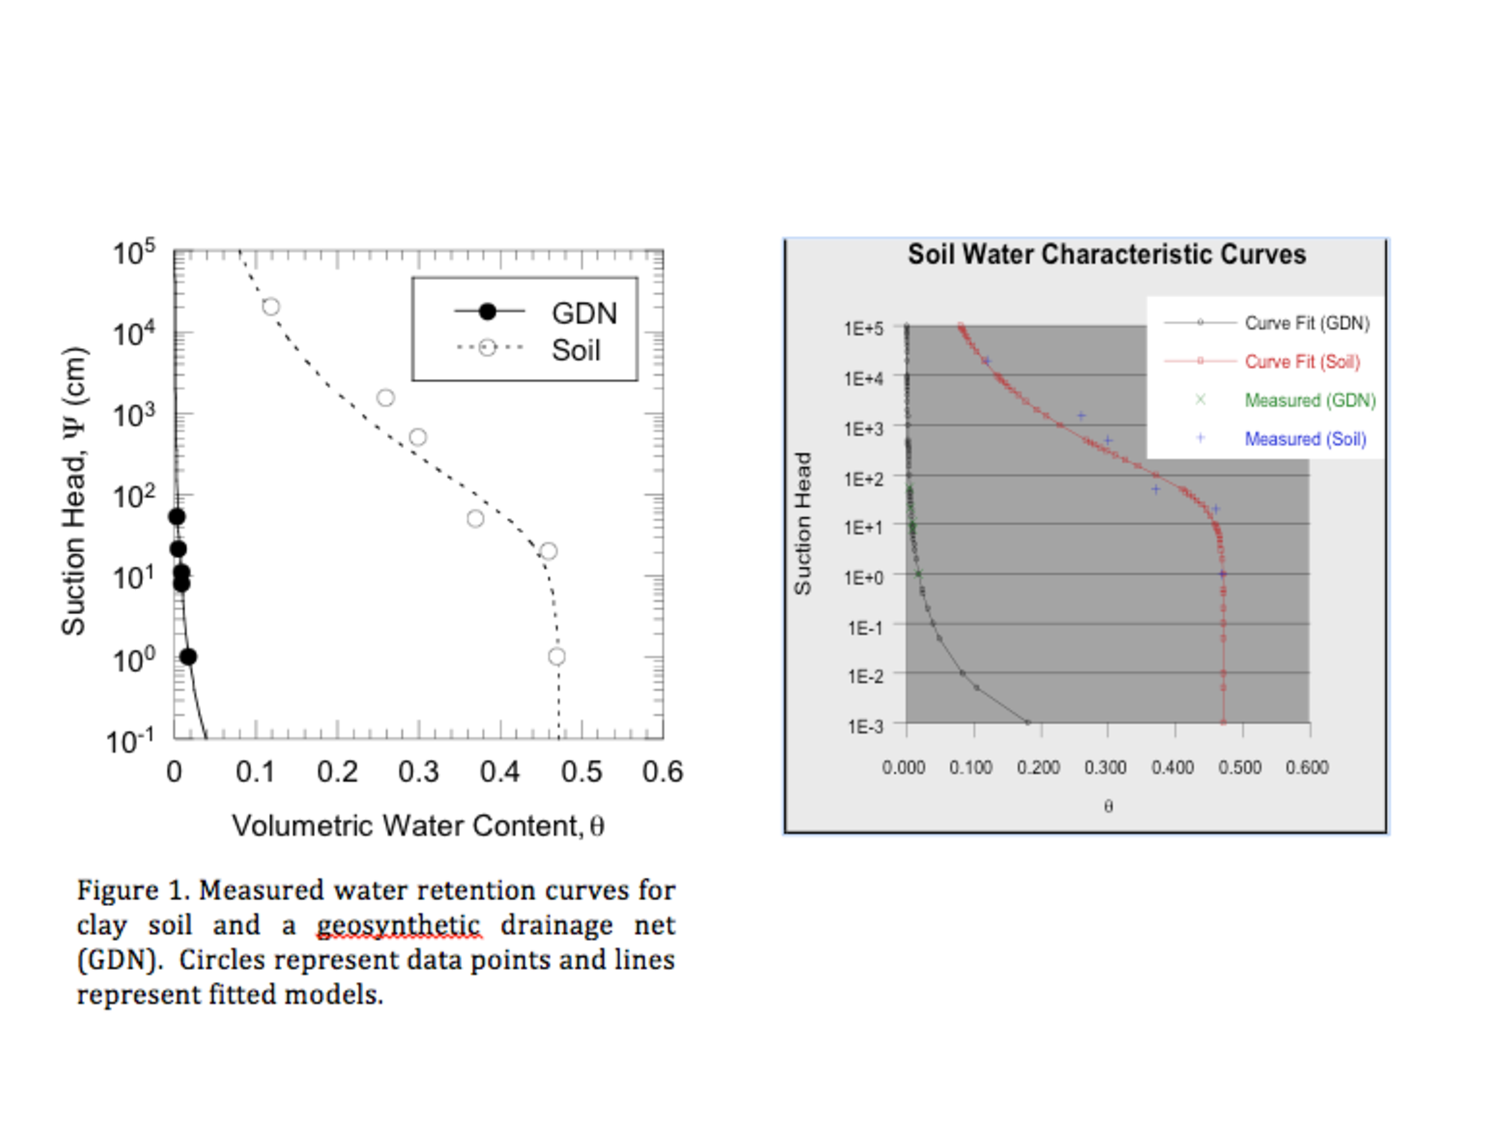
\includegraphics[width=1\textwidth]{soil_good_bad}
%\label{fig:awesome_image}
%\end{figure}

%\begin{figure}[!t]
%\centering
%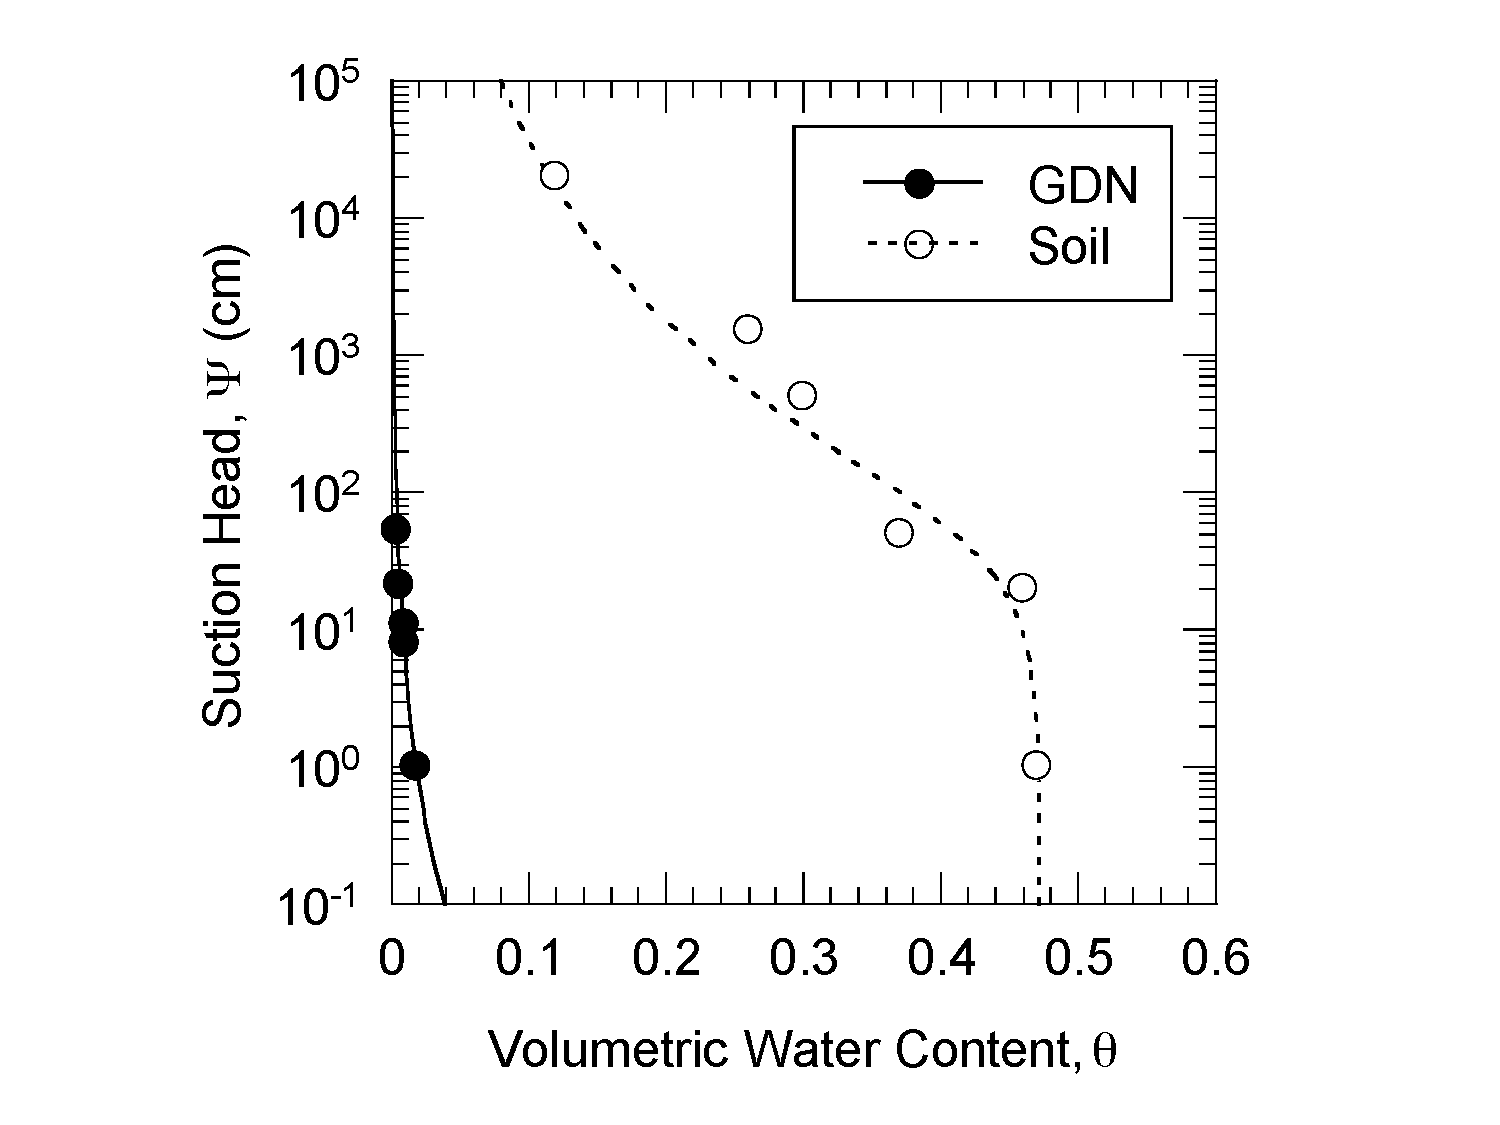
\includegraphics[width=0.6\textwidth]{Soil_good}
%\caption{Measured water retention curves for clay soil and a geosynthetic drainage net (GDN).  Circles represent data points and lines represent fitted models.}
%\end{figure}
%
%\begin{figure}[!t]
%\centering
%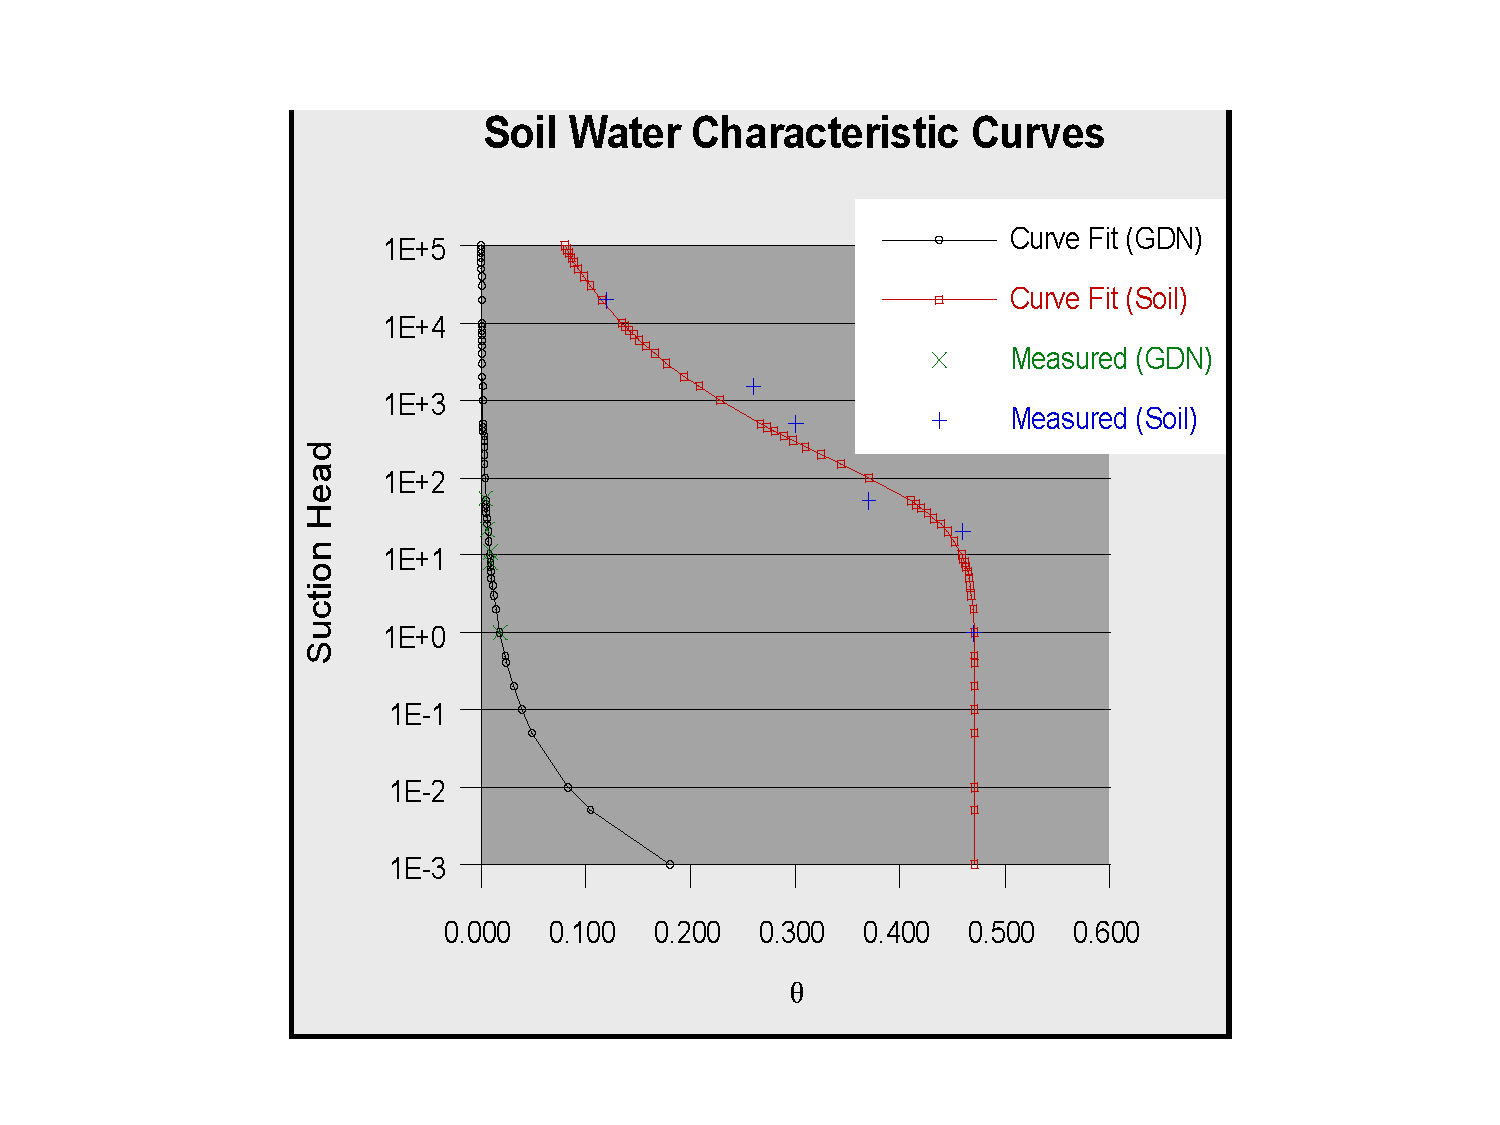
\includegraphics[width=0.6\textwidth]{Soil_notsogood}
%\end{figure}

%\pagebreak

%\begin{figure}[t]
%  \begin{minipage}{0.5\linewidth}
%  
%    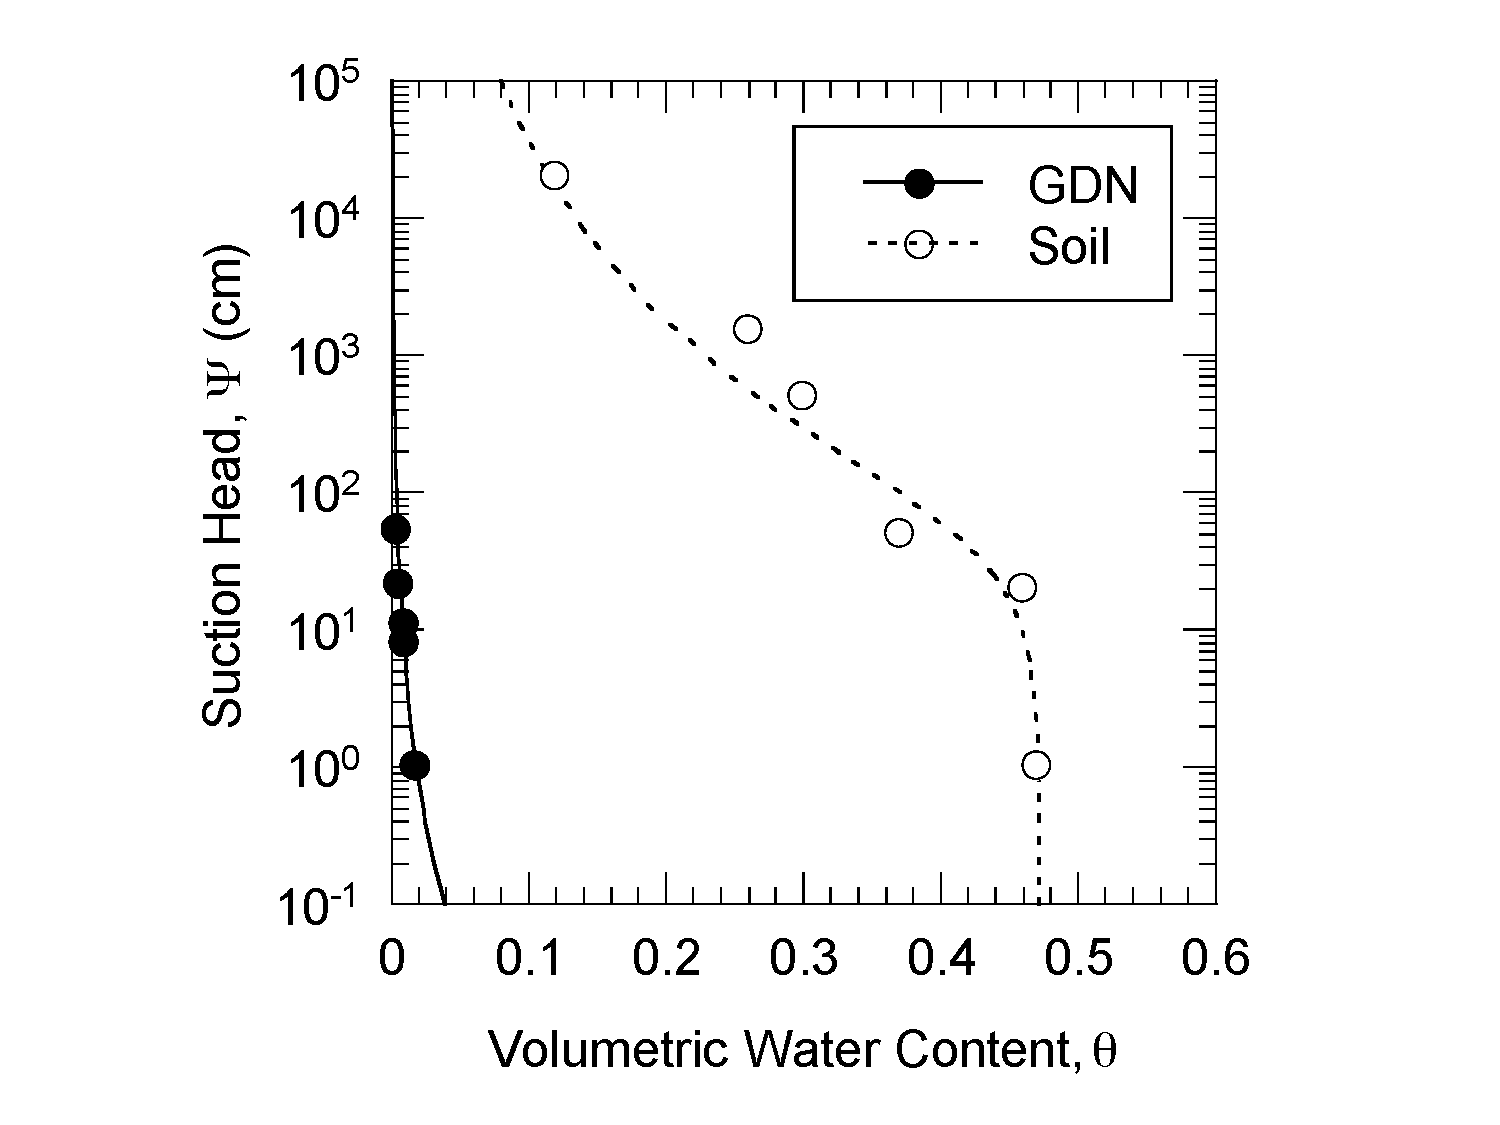
\includegraphics[width=1.2\textwidth]{Soil_good}
%    \caption{Measured water retention curves for clay soil and a geosynthetic drainage net (GDN). Circles represent data points and lines represent fitted models.}
%    \label{fig_good}
%  \end{minipage}%
%  \begin{minipage}{0.5\linewidth}
%    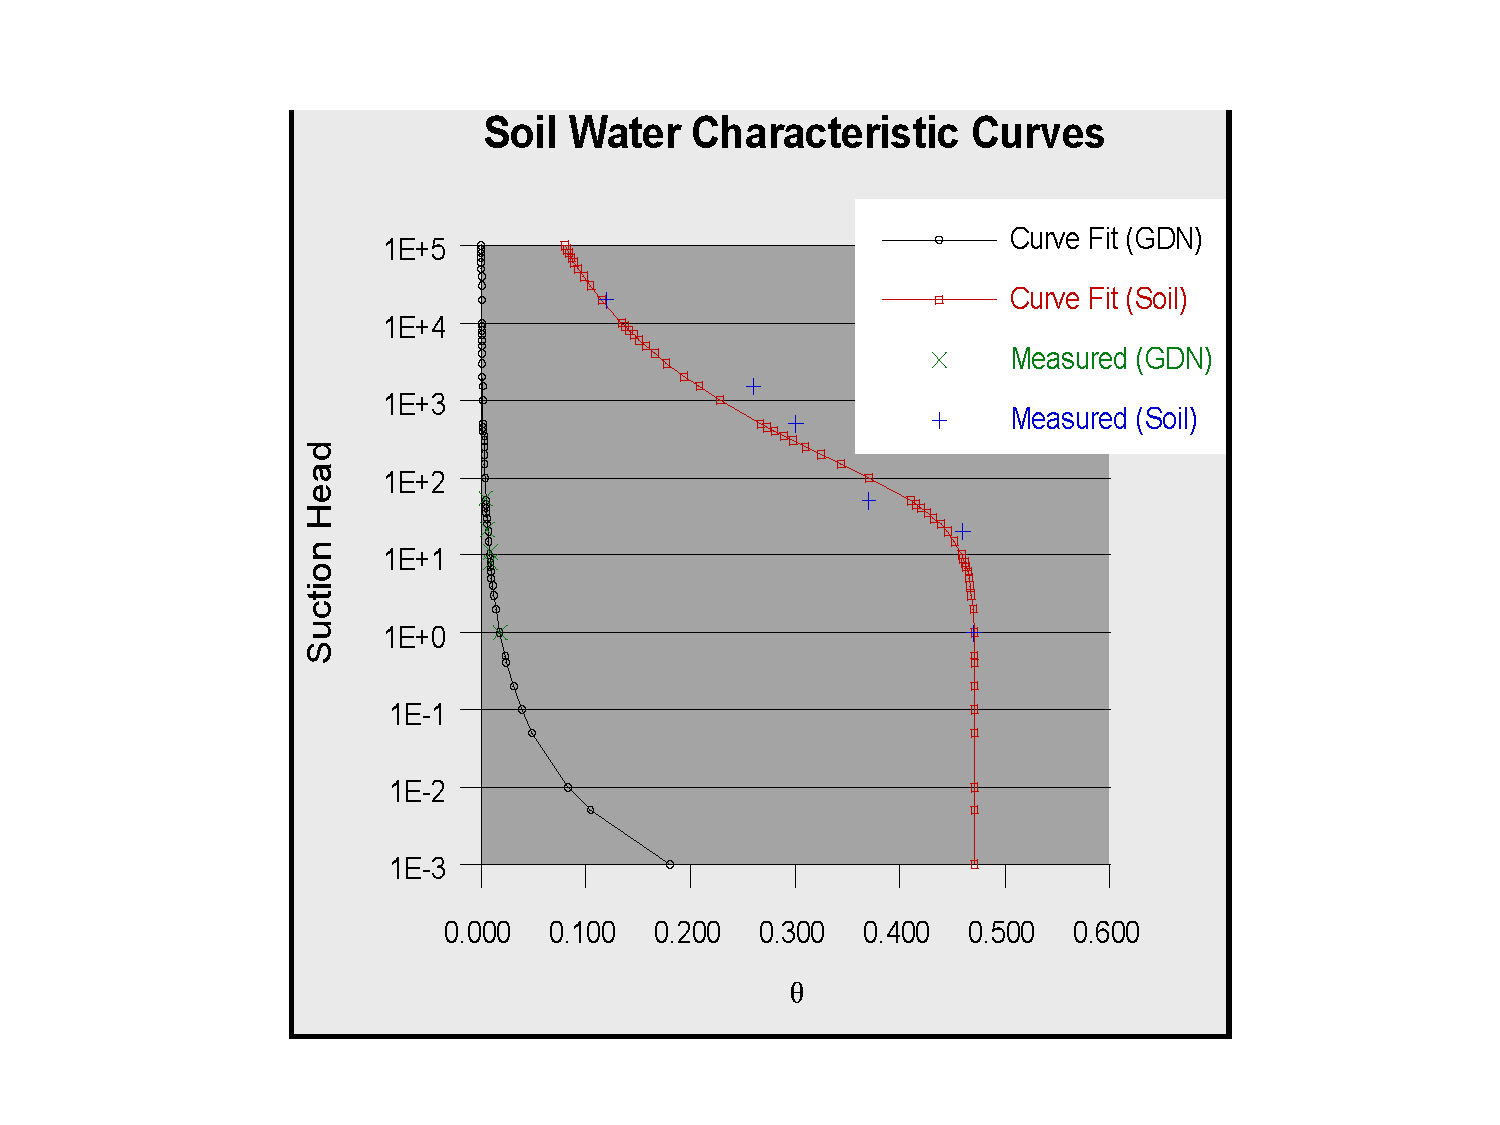
\includegraphics[width=1.2\textwidth]{Soil_notsogood}
%    \caption{The caption for figure 2.}
%    \label{fig_bad}
%  \end{minipage}
%\end{figure}
%
%\begin{figure}
%        
%        \begin{subfigure}[t]{0.45\linewidth}
%                \centering
%                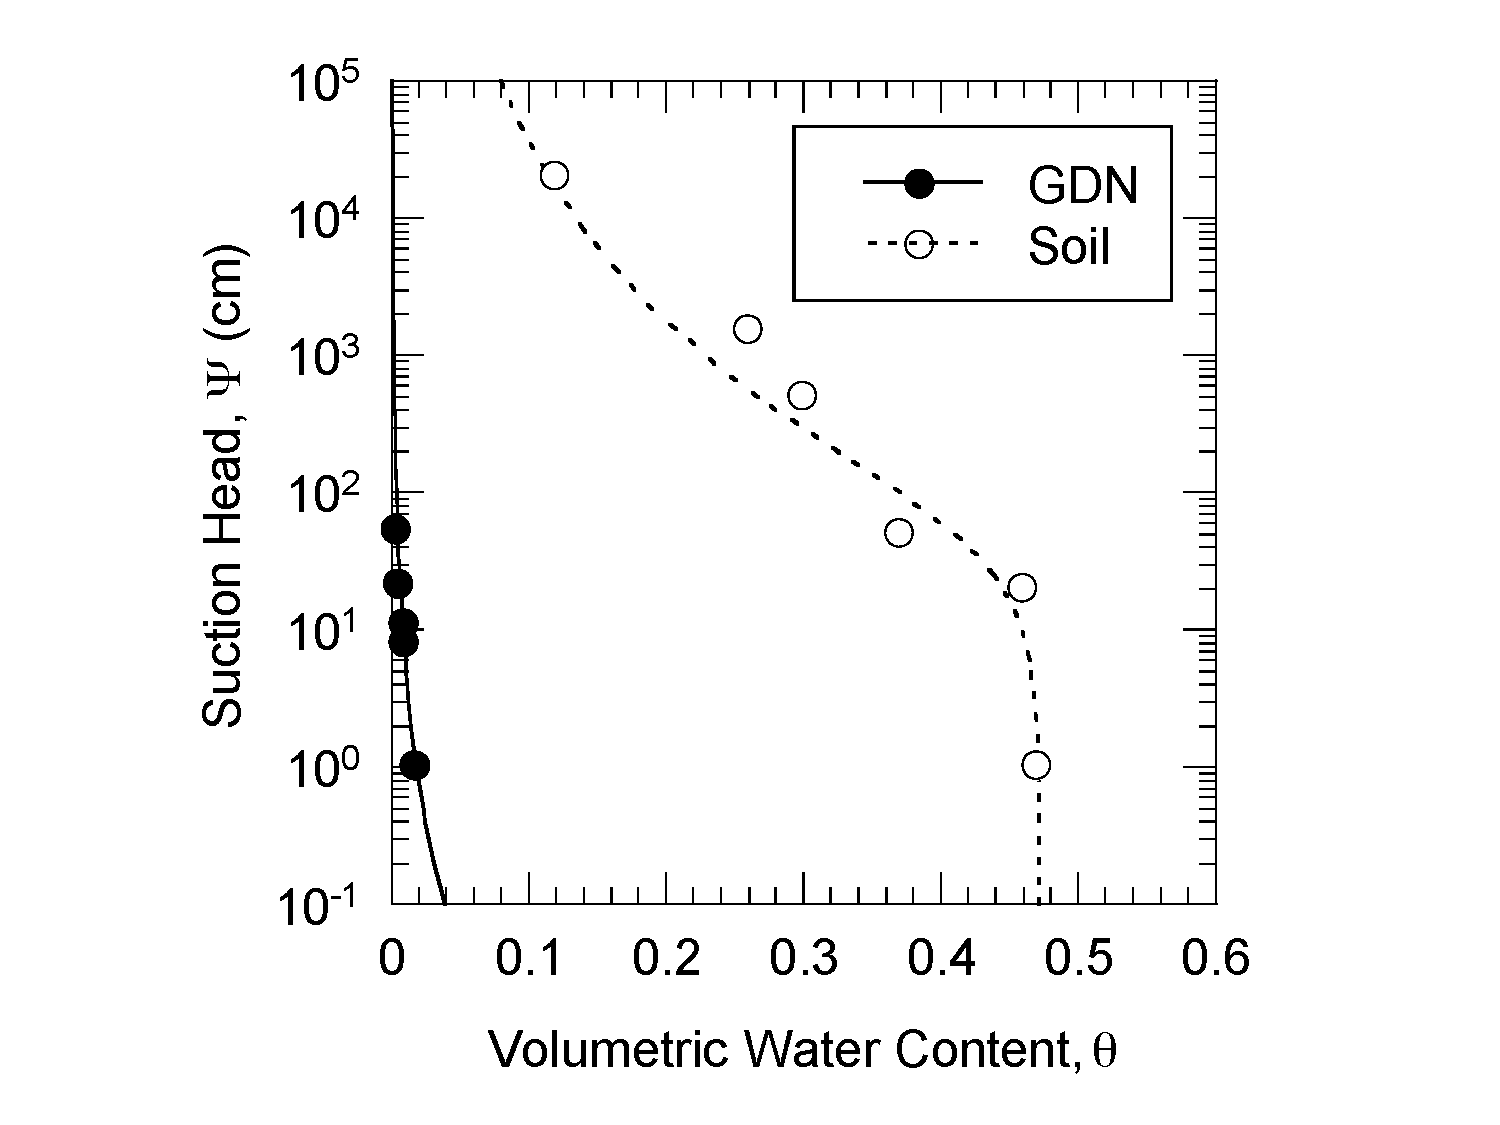
\includegraphics[width=1.2\textwidth]{Soil_good}
%                \centering
%                \caption{Measured water retention curves for clay soil and a geosynthetic drainage net (GDN). Circles represent data points and lines represent fitted models.}
%                \label{fig:hydrothermal}
%        \end{subfigure}
%        \hfill
%        \begin{subfigure}[t]{0.45\linewidth}
%                \centering
%                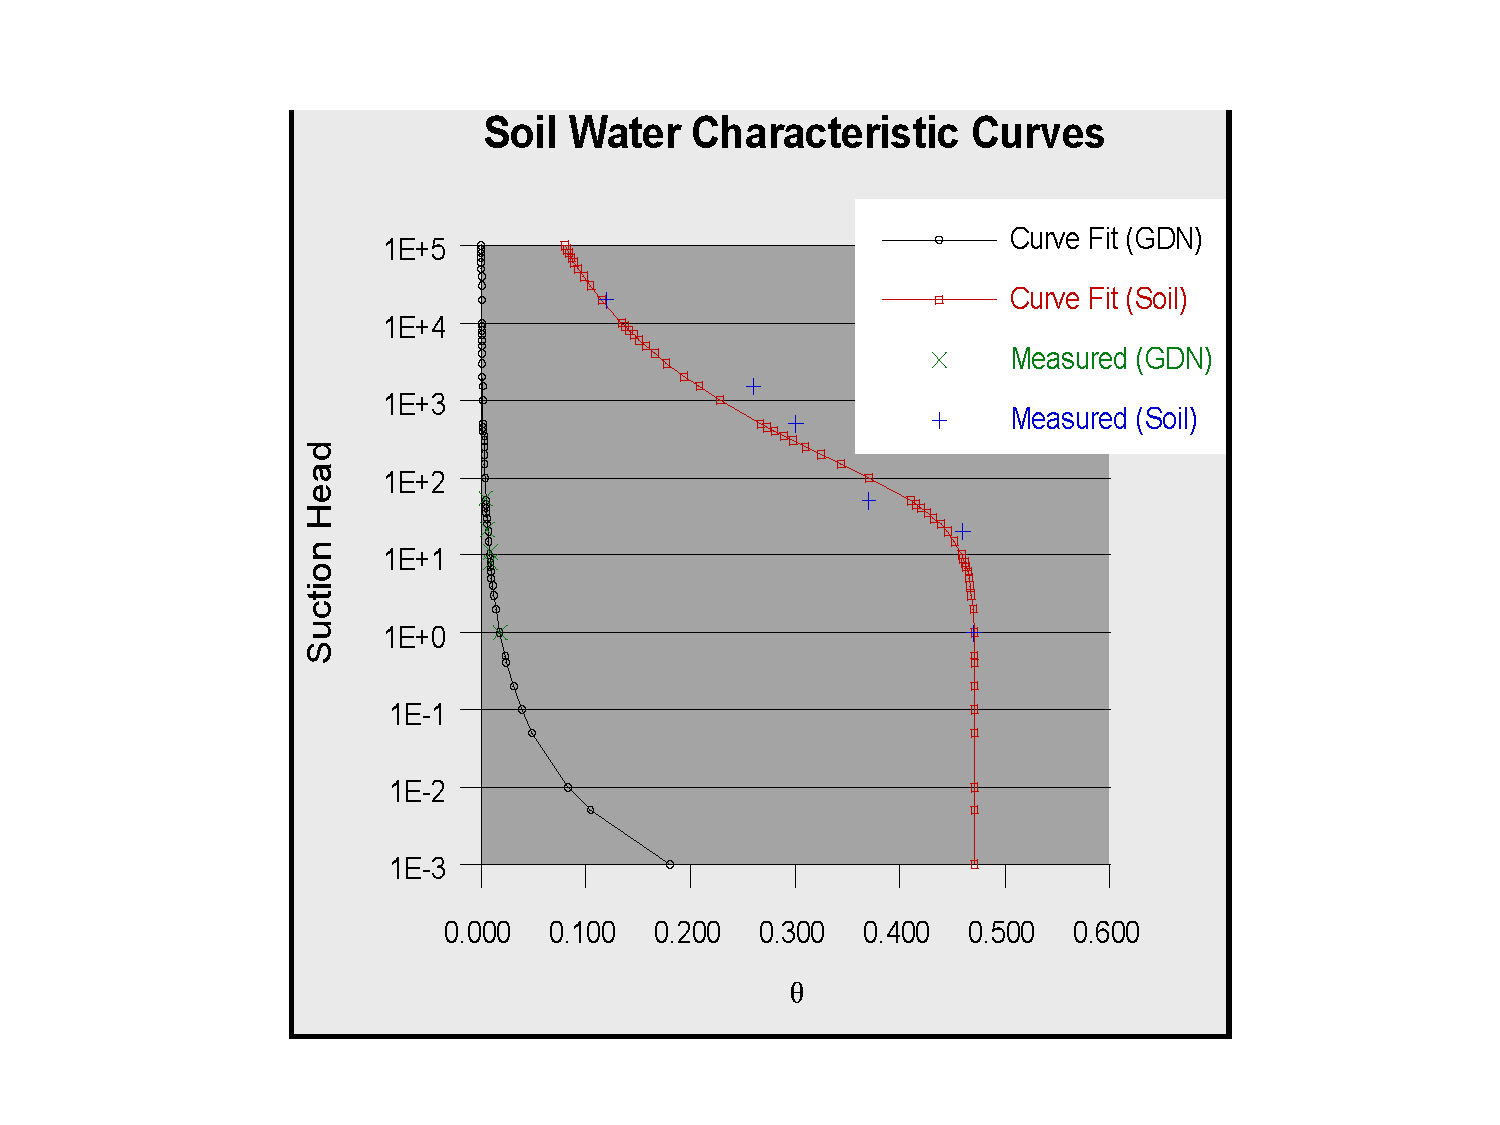
\includegraphics[width=1.2\textwidth]{Soil_notsogood}
%                \label{fig:EGS}
%        \end{subfigure}
%\end{figure}

\begin{figure} 
%% LARGER SUBFIGURE 
	\subfloat[Caption large box]{% 
		\begin{minipage}[c][1\width]{% 
			0.5\textwidth} \centering%	 
			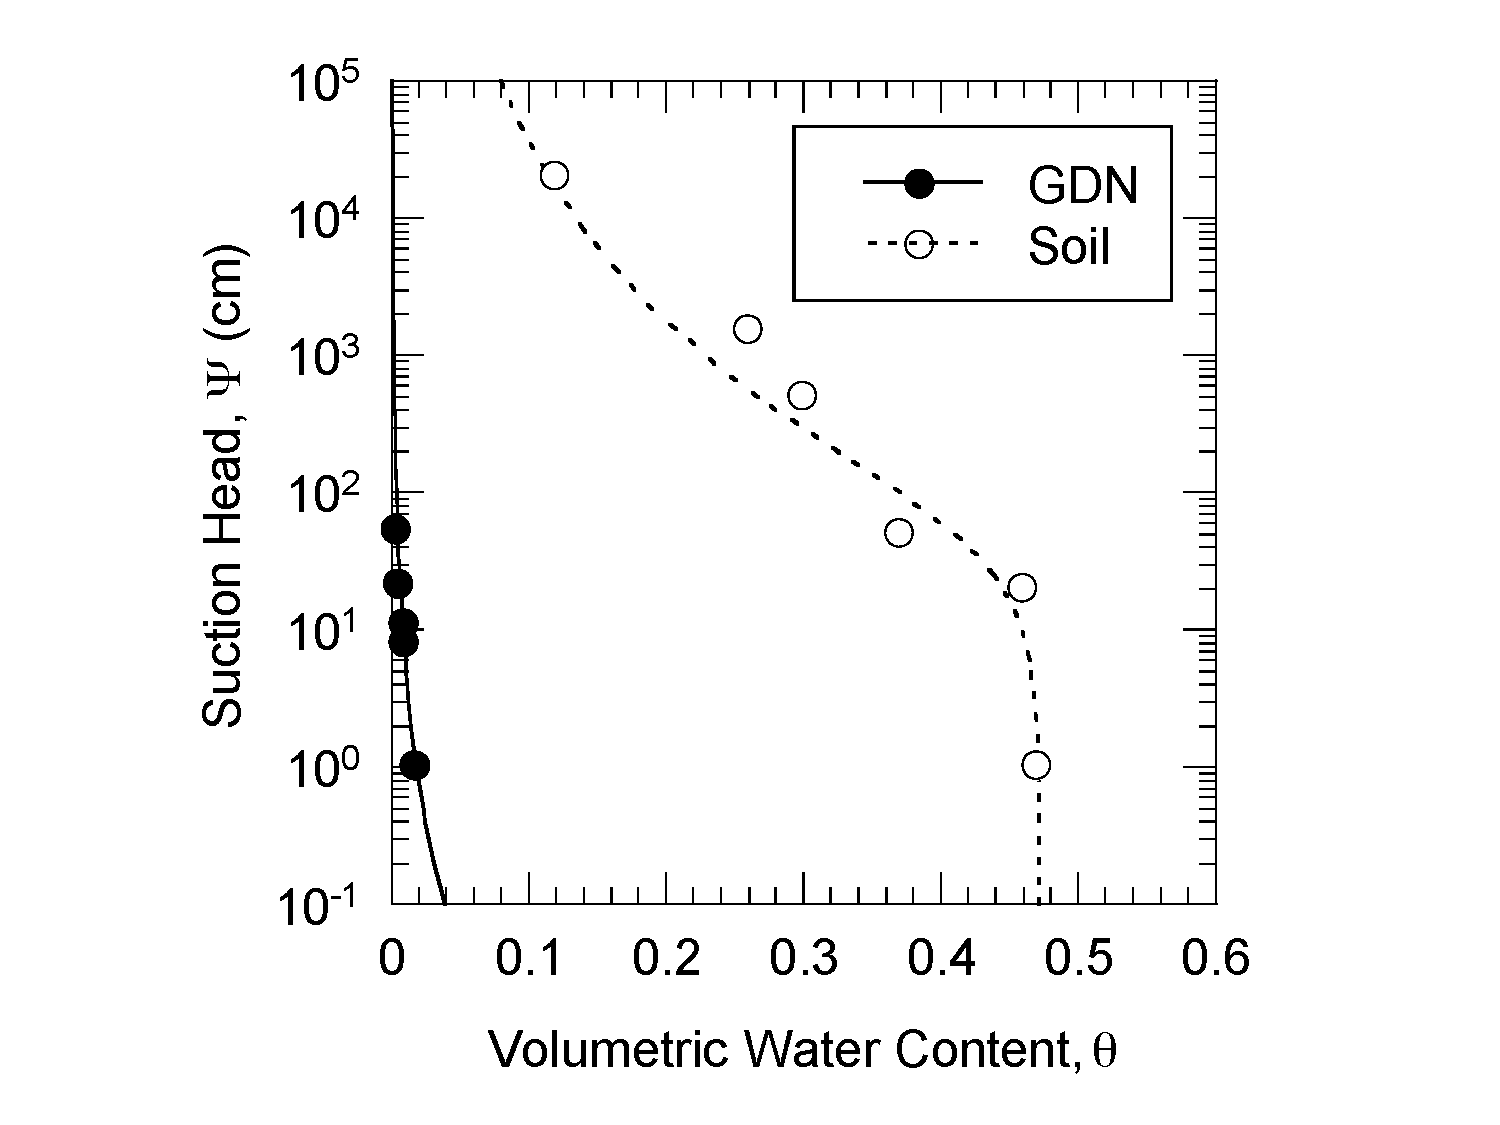
\includegraphics[width=0.8\textwidth]{Soil_good} 			 		
			\end{minipage}} 
			
%% SMALLER SUBFIGURE 
	\subfloat{% 
		\begin{minipage}[c][1\width]{% 
			0.5\textwidth}  \centering% 
		 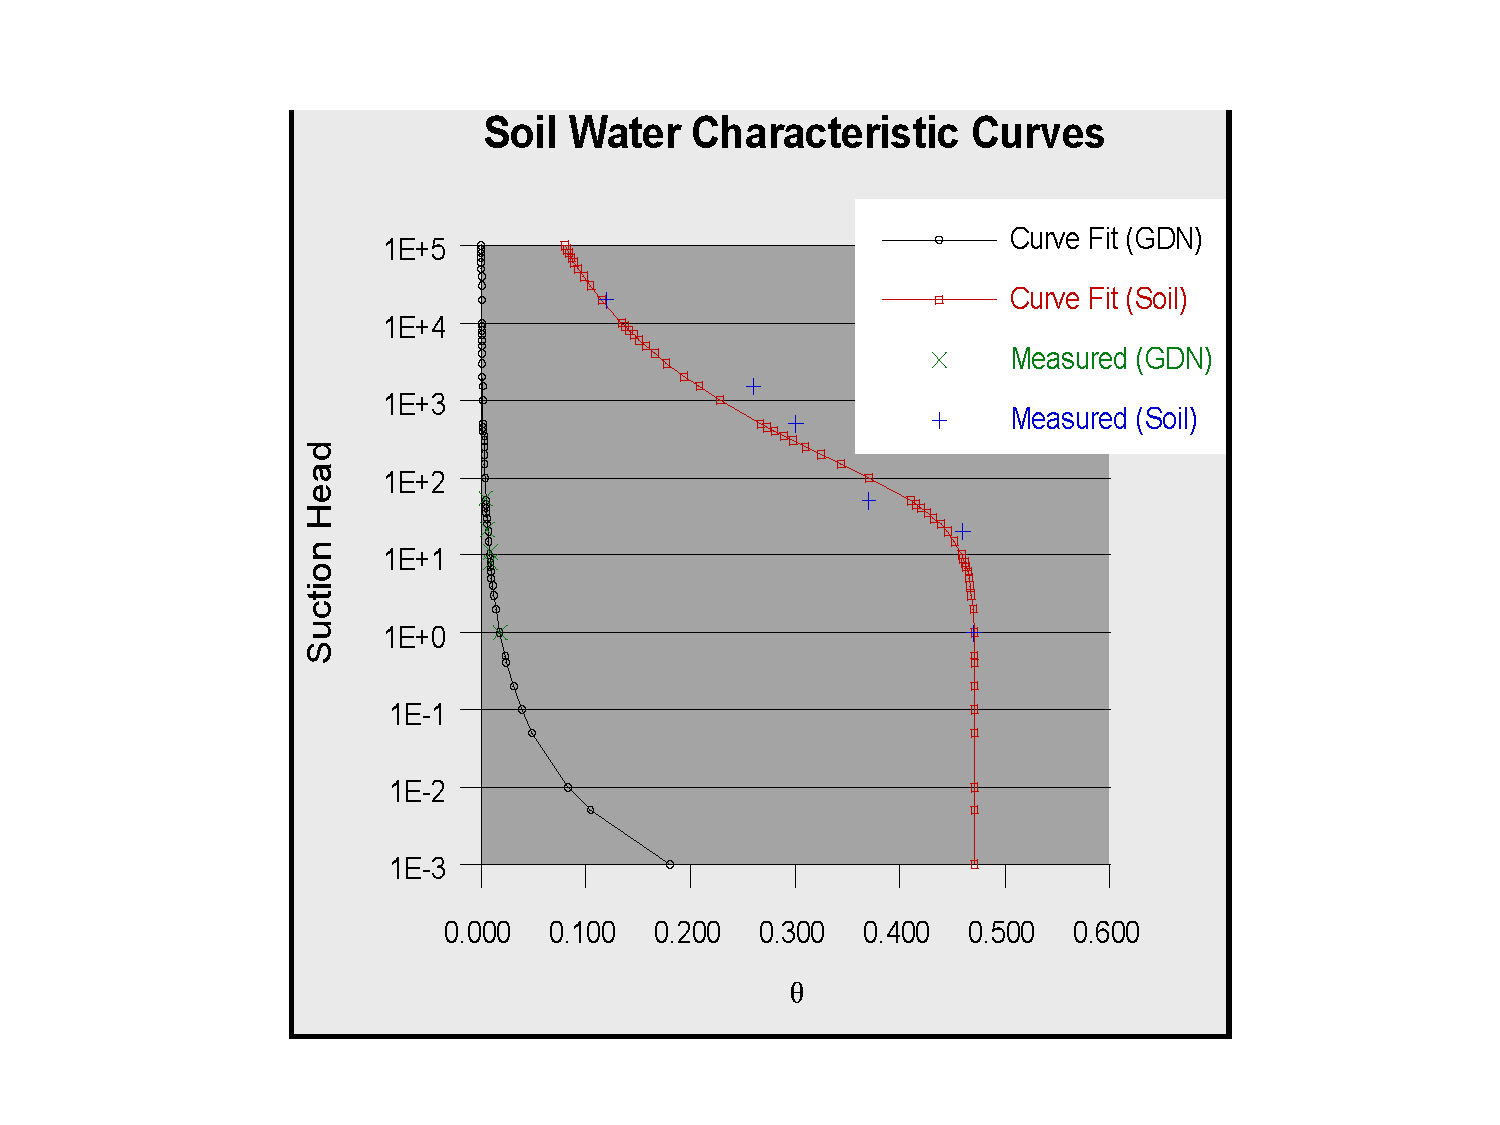
\includegraphics[width=0.8\textwidth]{Soil_notsogood} 		   
		 \end{minipage}} 
		 
\end{figure} 


Look at both figures and write down which figure is more effective and why. As you think about the quality of the figures, consider the following: Can you understand the point the author was trying to make with the figure? Does the figure stand on its own?  Are the numbers and labels on each axis clear and easy to understand?  Can you easily differentiate between the data and the fitted models? How would you improve the figure? [2 min]\\\\\\\\\\\\\\\\\\\\

Now discuss your thoughts in groups of three. One member of your group should take notes so you can report back to the rest of the class. [3--5 min] 

\section *{Model Fitting: Sorption}

%\subsection {Background}
\subsection *{Background}
Chlordane is a highly toxic chemical that was used widely as an insecticide until it was banned in the U.S. in the late 1980s \cite{army2009}.  Athough it was banned over 25 years ago, chlordane is still detected in groundwater in rural parts of the U.S. \cite{bidel2004}, and treating chlordane-contaminated water is challenging.

\subsection *{Problem Description}
The influent water to a drinking water plant in Ames, Iowa is contaminated with the insecticide chlordane. The plant operator has contracted the firm you work for to design a  process to remove chlordane from the water. The firm is considering designing a treatment process that uses granulated activated carbon (GAC).\\

You are part of a team that has been asked to asses whether treating the water with GAC will reduce chlordane concentrations to below its maximum contaminant level of 2 ppb. Your supervisor has asked you and the other new engineer in the firm to conduct a set of experiments to determine the parameters for the sorption isotherm of chlordane on GAC.  The model  parameters will be used to design a bench-scale treatment unit that will be further tested.\\

Your coworker conducted the laboratory study and collected the data. You have to fit the data to two isotherms---Linear and Freundlich described in Eq. 1 and Eq. 2, respectively, and send a preliminary memo to your co-worker.  She has kindly agreed to write up the complete memo and send it to your supervisor.\\

\begin{equation}
q = KC
\end{equation}


\begin{equation}
q = KC^{\sfrac{1}{n}}
\end{equation}\\

where q = mass of adsorbate adsorbed per mass of adsorbent at equilibrium ($\sfrac{mg}{g}$),\\

C = concentration of adsorbate in the aqueous phase at equilibrium ($\sfrac{mg}{L}$),\\

K = Freundlich isotherm capacity parameter (($\sfrac{mg}{g}$)($\sfrac{L}{mg})^{\sfrac{1}{n}}$), and\\

$\sfrac{1}{n}$ = Freundlich isotherm intensity parameter (unitless).\\

%In addition, you need to send a preliminary memo to your co-worker that describes the modeling work you have done.  In this introductory memo you should include the methods (e.g. description of the software package and equations you used), your figure, and a discussion of the figure.  

\subsection *{Assignment}

A data file (Excel) titled ``Sorption Data'' is located at blahblahblah drive blah
%/ facultystaff on ‘netspace’ (T:)/dls054/public/CENG340/Week5_LabFiles/.  
The file contains one data set of dissolved chlordane concentration, C$_{aq}$ (mg/L), vs adsorbed chlordane concentration, C$_{adsorbed}$ (mg/[g GAC]).

\begin{itemize} 
\item Use KaleidaGraph (or another software package of your choice) to fit the data set to  the two isotherm models---linear and Freundlich.
\item Create one high-quality plot with the C$_{aq}$ vs. C$_{adsorbed}$ data points, and the two curves that illustrates the model fits to the data set. 
\item Think about how well each model fits the data and which model you think is most  appropriate. Note that we will not conduct proper statistical tests for goodness of fit, but you should be able to visually assess which model best fits the data and discuss this in your memo.
 
\end{itemize}


\subsection *{Deliverables}
Summarize your work in a preliminary memo addressed to your co-worker. For this assignment include the following sections: (1) Objective, (2) Methods,(3) Results and Discussion (this is where you will include the figures you created).  For this exercise you do not need to include Introduction and Conclusion sections.\\

Refer to the instructions handed out at the beginning of the semester for  formatting and writing style, and the sample memo.\\




\begin{thebibliography}{9}


\bibitem{army2009}

Medina, Victor F and Waisner, Scott A and Morrow, Agnes B and Butler, Afrachanna D and Johnson, David R and Harrison, Allyson and Nestler, Catherine C,
``Legacy chlordane in soils from housing areas treated with organochlorine pesticides,''
\emph{US Army Corps of Engineers}, 2009.

\bibitem{bidel2004}

Bidleman, Terry F and Wong, Fiona and Backe, Cecilia and S{\"o}dergren, Anders and Brorstr{\"o}m-Lund{\'e}n, Eva and Helm, Paul A and Stern, Gary A,
``Chiral signatures of chlordanes indicate changing sources to the atmosphere over the past 30 years,''
\emph{Atmospheric Environment}, vol. 38, pp. 5963--5970, 2004.

 

\end{thebibliography}
\pagebreak
\section *{In Class Exercise 2: Brainstorming and Drafting}
\begin{enumerate}
\item Take a few minutes and fill out the following page with ideas for your memo.  If you use a laptop, don't worry about wording, sentence structure, or grammar. [15 minutes]\\ 

\textbf{Objective}\\\\\\\\\\\\\\\\

\textbf{Methods}\\\\\\\\\\\\\\\\\\\\

\textbf{Results and Discussion}\\\\\\\\\\\\\\\\\\\\\\\\\\\\\\\\

\item Share your thoughts with a partner.  Discuss what information belongs in each section. and how you will describe and analyze the figure you created.  Be prepared to share your ideas with the larger group. [5 minutes]
\end{enumerate}


\end{document}